\documentclass[11pt]{article}
\usepackage[margin=1in]{geometry}
\usepackage{amsmath,amssymb}
\usepackage{booktabs}
\usepackage{float}
\usepackage{graphicx}
\usepackage{xcolor}
\usepackage{hyperref}
\usepackage{enumitem}
\usepackage{caption}
\usepackage[most]{tcolorbox}
\usepackage{tikz}
\usetikzlibrary{arrows.meta,positioning,fit,backgrounds}
\hypersetup{colorlinks=true, linkcolor=blue, citecolor=blue, urlcolor=blue}
\captionsetup{font=small,labelfont=bf}

\definecolor{good}{HTML}{1F7A4D}
\definecolor{bad}{HTML}{B23B3B}
\definecolor{accent}{HTML}{8A5A2B}
\definecolor{oracle}{HTML}{2F6FB0}
\newtcolorbox{keybox}{colback=orange!5,colframe=orange!55,breakable,
  left=6pt,right=6pt,top=5pt,bottom=5pt}

% ---- result macros (single source of truth for every number) --------------
% tokenizer / world model (measured, Stage A/A2)
\newcommand{\reconMSE}{0.0156}
\newcommand{\activeAfter}{256}
\newcommand{\wmTok}{97.8}
\newcommand{\wmRew}{99.1}
\newcommand{\wmDone}{99.1}
% ball-recall ablation (11 seeds). Reliability = # seeds preserving the ball.
\newcommand{\nseeds}{11}
\newcommand{\keptPlain}{4}
\newcommand{\keptEMA}{2}
\newcommand{\keptFG}{11}
\newcommand{\recallPlain}{0.35}      % plain VQ + uniform, mean ball recall
\newcommand{\recallEMA}{0.16}        % EMA + uniform, mean ball recall
\newcommand{\ballFG}{1.00}           % EMA + fg-weighted, ball recall (11/11 seeds)
\newcommand{\activePlain}{8}         % active codes, plain VQ (collapsed)
\newcommand{\activeEMA}{254}         % active codes, EMA + uniform (healthy)
\newcommand{\activeFG}{256}          % active codes, EMA + fg-weighted (healthy)
\newcommand{\reconPlain}{0.014}      % recon MSE, plain VQ
\newcommand{\reconEMA}{0.021}        % recon MSE, EMA + uniform
\newcommand{\reconFGtab}{0.000}      % recon MSE, EMA + fg (ablation, 2000 steps)
\newcommand{\reconFG}{2\times10^{-6}} % near-perfect recon MSE (deployed tokenizer, 2500 steps)
\newcommand{\activeDeployed}{251}    % active codes of the deployed win tokenizer
\newcommand{\wmParams}{3.34}
\newcommand{\tokParams}{0.83}
\newcommand{\acParams}{0.82}
% policy / evaluation (measured, Stage B — 500 real episodes)
\newcommand{\catchRate}{1.00}
\newcommand{\catchReturn}{+1.0}
\newcommand{\randCatch}{0.16}
\newcommand{\randReturn}{-0.68}
\newcommand{\wmFidelity}{0.0047}
\newcommand{\nrounds}{one}

\title{\textbf{Dream to Catch}\\[2pt]
\large Building an IRIS World Model from Scratch, Diagnosing Two Coupled
Failures, and Learning to Play in Imagination}
\author{Vizuara AI Labs \\ \small RL-in-Production Bootcamp --- Project 2}
\date{\today}

\begin{document}
\maketitle

\begin{abstract}
Model-based reinforcement learning promises to let an agent learn a task by
\emph{practising in a learned simulator} rather than in the real environment.
\textbf{IRIS}~\cite{iris} is the Atari-scale realization of this idea: it
discretizes each frame into a short sequence of tokens and models the
environment with a next-token Transformer, exactly like a language model. We
reimplement all three IRIS components \emph{from scratch}---a VQ-VAE
tokenizer, an autoregressive Transformer world model, and an actor-critic
trained \emph{purely in imagination}---and study them on a deterministic pixel
``Catch'' task, run on a single A10G GPU via Modal. Naively assembled, the agent
plays at random. We trace the failure backwards: the policy gets no gradient
because its dream contains no ball, because the tokenizer drops the ball. A
controlled ablation then \emph{disentangles two independent pathologies} that
are usually conflated. The first is textbook VQ-VAE codebook collapse (the plain
codebook uses $\approx\activePlain$ of 256 codes). The second---and the actual
reason the ball vanishes---is that a background-dominated reconstruction loss
under-weights the tiny bright ball: under a uniform loss the ball survives in
only \keptEMA{} of \nseeds{} seeds \emph{even with a fully healthy \activeAfter-code
codebook}. We fix the first with EMA codebook updates and dead-code
revival~\cite{vqvae2,jukebox}, and the second with a foreground-weighted
reconstruction loss---a cheap stand-in for the perceptual term IRIS uses and the
base implementation had dropped---which preserves the ball on all
\keptFG/\nseeds{} seeds (recall \ballFG). With the ball restored, the dream
finally contains something to catch, and the actor-critic---trained \emph{only}
inside that dream---learns to play: real-environment catch rate \textbf{\catchRate}
versus a random baseline of \randCatch{} and an oracle of $1.0$. The lesson generalizes beyond Catch:
\emph{a world model can only teach a policy what its tokenizer chooses to
preserve, and a uniform reconstruction loss quietly chooses to discard exactly
the small, fast, task-critical objects.}
\end{abstract}

%============================================================================
\section{Introduction}
\label{sec:intro}
%============================================================================
A \textbf{world model} is a learned simulator of an environment: given the
current observation and an action, it predicts the next observation, the reward,
and whether the episode terminates. Its appeal is sample efficiency---once the
model is good enough, a policy can be trained on \emph{imagined} experience,
never touching the (expensive, slow, or unsafe) real environment. This
``learning in a dream'' lineage runs from Ha \& Schmidhuber's \emph{World
Models}~\cite{worldmodels} through DeepMind's \emph{Dreamer}
family~\cite{dreamer,dreamerv2,dreamerv3}. \textbf{IRIS}~\cite{iris} is the
version that scales the idea to pixels by making the world model a
\emph{language model over image tokens}: a discrete autoencoder turns each frame
into a small set of tokens from a fixed codebook, and an autoregressive
Transformer predicts the environment one token at a time.

We rebuild all three IRIS components \emph{from scratch}---no \texttt{iris}
library---and study them on a task small enough that every moving part is
visible: a deterministic pixel \emph{Catch}, where a paddle must intercept a
falling ball. The point is diagnostic. Assembled naively, the agent plays at
random, and the interesting question is \emph{why}. Tracing the failure
backwards, the actor-critic gets no useful gradient because the world model's
dream contains no ball to catch, because the tokenizer discards the ball from
every frame. The usual explanation for a discarded object is VQ-VAE
\emph{codebook collapse}. We show that this explanation, while pointing at a real
pathology, is \emph{incomplete}---and in isolating what it misses we recover a
working agent.

\paragraph{Contributions.}
\begin{enumerate}[leftmargin=1.4em,itemsep=1pt,topsep=2pt]
\item A faithful, dependency-free \textbf{from-scratch IRIS}---VQ-VAE tokenizer,
  autoregressive Transformer world model, and an actor-critic trained
  \emph{purely in imagination}---that runs end-to-end on a single A10G GPU via
  Modal for a few dollars, with every component exposed and configurable.
\item A controlled ablation that \textbf{disentangles two independent tokenizer
  pathologies} usually conflated. (i)~\emph{Codebook collapse}: plain VQ uses
  only $\approx\!\activePlain$ of $256$ codes; fixed with EMA codebook updates
  and dead-code revival~\cite{vqvae2,jukebox}. (ii)~The \emph{actual} reason the
  ball vanishes: a background-dominated reconstruction loss under-weights the
  tiny bright ball, so under a uniform loss ball preservation is an unreliable
  coin-flip \emph{even with a fully healthy \activeAfter-code codebook}
  ($\keptEMA/\nseeds$ seeds). We fix this with a foreground-weighted
  reconstruction loss---a cheap stand-in for the perceptual term IRIS uses and
  the base implementation had dropped---which preserves the ball on
  $\keptFG/\nseeds$ seeds.
\item With the ball restored (recall $\approx\!\ballFG$), the dream finally
  contains something to catch, and the imagination-trained actor-critic
  \textbf{learns to play}: real-environment catch rate \catchRate{} versus a
  random baseline of \randCatch{} and an oracle of $1.0$.
\end{enumerate}

The lesson generalizes beyond Catch: \emph{a world model can only teach a policy
what its tokenizer chooses to preserve, and a uniform reconstruction loss
quietly chooses to discard exactly the small, fast, task-critical objects.}

%============================================================================
\section{Background and Related Work}
\label{sec:related}
%============================================================================
Learning to act inside a learned model of the environment traces back to
\emph{World Models}~\cite{worldmodels}, which trained an unsupervised generative
model of an RL environment and showed that a controller could be optimized
entirely within its ``dream'' rollouts. The \emph{Dreamer} family scaled this
into a practical latent-imagination agent: Dreamer~\cite{dreamer} learned
long-horizon visual-control behaviours by propagating value gradients through
imagined latent trajectories; DreamerV2~\cite{dreamerv2} replaced the continuous
latent with \emph{discrete} representations and reached human-level Atari
performance; and DreamerV3~\cite{dreamerv3} generalized the recipe across more
than 150 tasks with a single configuration. \textbf{IRIS}~\cite{iris} departs
from these recurrent latent models by casting the world model as an
autoregressive Transformer over discrete image tokens produced by a discrete
autoencoder, achieving strong sample efficiency on Atari 100k---a benchmark also
targeted by the pixel-level model-based agent SimPLe~\cite{simple}.

The discrete-token backbone IRIS reuses originates in VQ-VAE~\cite{vqvae}, whose
vector-quantized codebook (with a commitment loss and an EMA codebook-update
variant) supplies the discrete image codes; VQ-VAE-2~\cite{vqvae2} extended this
to hierarchical, EMA-trained codebooks for high-fidelity generation. A
well-documented failure mode of these codebooks is \emph{collapse} onto a few
active codes, which we address with the random-restart / codebook-reset
heuristic introduced for audio VQ in Jukebox~\cite{jukebox}, where under-used
embeddings are periodically reset to encoder outputs from the current batch. We
evaluate on a pixel version of the \emph{Catch} task popularized by the
Behaviour Suite for RL (bsuite)~\cite{bsuite}. Our contribution is not a new
algorithm but a precise, reproducible dissection: on a task small enough to see
every moving part, we show that the commonly-cited ``codebook collapse''
diagnosis is \emph{insufficient} to explain a dropped object, and we isolate the
reconstruction-loss geometry as the true cause.

%============================================================================
\section{The Three Components, From Scratch}
\label{sec:components}
%============================================================================
IRIS factorizes a pixel agent into three learned modules
(Fig.~\ref{fig:pipeline}): a discrete autoencoder that turns frames into tokens,
an autoregressive Transformer that predicts those tokens, and an actor-critic
that learns from the Transformer's rollouts. We reimplement each faithfully and
expose every dimension as a config knob.

\begin{figure}[H]\centering
\scalebox{0.92}{%
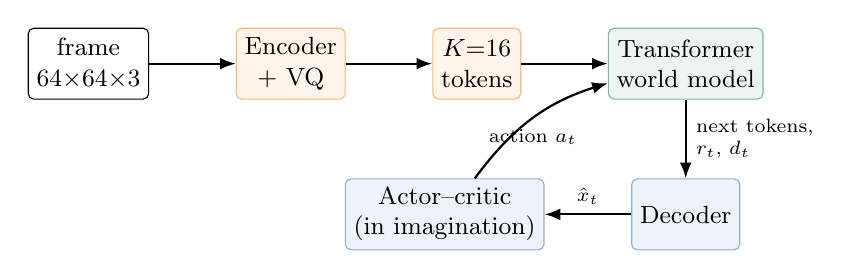
\begin{tikzpicture}[
  node distance=6mm and 11mm, font=\small,
  box/.style={draw, rounded corners=2pt, minimum height=9mm, align=center,
    inner sep=3pt, fill=white},
  tok/.style={box, fill=orange!8, draw=orange!55},
  wm/.style={box, fill=good!8, draw=good!55},
  ac/.style={box, fill=oracle!8, draw=oracle!55},
  ar/.style={-{Latex[length=2mm]}, thick}]
  \node[box] (frame) {frame\\$64{\times}64{\times}3$};
  \node[tok, right=of frame] (enc) {Encoder\\+ VQ};
  \node[tok, right=of enc] (tokens) {$K{=}16$\\tokens};
  \node[wm, right=of tokens] (wm) {Transformer\\world model};
  \node[ac, below=10mm of wm] (dec) {Decoder};
  \node[ac, left=of dec] (ac) {Actor--critic\\(in imagination)};
  \draw[ar] (frame) -- (enc);
  \draw[ar] (enc) -- (tokens);
  \draw[ar] (tokens) -- (wm);
  \draw[ar] (wm) -- node[right,align=left,font=\scriptsize]{next tokens,\\ $r_t$, $d_t$} (dec);
  \draw[ar] (dec) -- node[above,font=\scriptsize]{$\hat x_t$} (ac);
  \draw[ar] (ac) to[bend left=18] node[below,font=\scriptsize]{action $a_t$} (wm);
\end{tikzpicture}}
\caption{The from-scratch IRIS pipeline. The tokenizer (orange) maps a frame to
$K$ discrete tokens; the Transformer world model (green) autoregressively
predicts the next frame's tokens, reward, and done; the actor-critic (blue)
observes decoded dream frames $\hat x_t=D(z_t)$ and its actions feed back into
the world model. During policy learning the real environment is never touched.}
\label{fig:pipeline}
\end{figure}

\paragraph{1. Tokenizer (VQ-VAE), 0.83\,M params.}
A convolutional encoder $E$ maps a $64{\times}64{\times}3$ frame to a
$4{\times}4$ latent grid; each cell $z_e$ is snapped to its nearest entry in a
learned codebook $\{e_i\}_{i=1}^{N}$ ($N{=}256$, dim $128$), giving $K{=}16$
discrete tokens, which a decoder $D$ maps back to pixels. The encoder is trained
through the straight-through estimator with a commitment loss, and reconstructed
with an $L_1$ objective:
\begin{equation}
\mathcal{L}_{\text{tok}} = \underbrace{\frac{\sum_{p} w_p\,\lVert x_p-\hat
x_p\rVert_1}{\sum_p w_p}}_{\text{reconstruction}}
\;+\; \beta\,\lVert z_e-\mathrm{sg}[e]\rVert_2^2,
\qquad w_p = 1 + \lambda_{\text{fg}}\max_c x_{p,c}.
\label{eq:tok}
\end{equation}
Two design choices are the subject of \S\ref{sec:results}. \emph{(a) Codebook
health.} Rather than learn the codebook through the usual code-book loss
$\lVert\mathrm{sg}[z_e]-e\rVert^2$ (which collapses onto a few codes), we update
it by an exponential moving average of the encoder vectors assigned to each
code~\cite{vqvae,vqvae2}, $N_i\!\leftarrow\!\gamma N_i+(1{-}\gamma)n_i$,
$m_i\!\leftarrow\!\gamma m_i+(1{-}\gamma)\!\sum z_e$, $e_i\!\leftarrow\!m_i/N_i$,
and periodically \emph{revive} any code with cluster size $N_i<1$ by resetting it
to a random encoder vector from the current batch~\cite{jukebox}. \emph{(b)
Foreground weighting.} The pixel weight $w_p$ in Eq.~\ref{eq:tok} upweights bright
pixels ($\lambda_{\text{fg}}{=}25$); with $\lambda_{\text{fg}}{=}0$ this reduces
to the base implementation's uniform $L_1$, which---as we show---fails to
reliably preserve the ball regardless of codebook health. This term is a
lightweight stand-in for the
perceptual reconstruction loss IRIS uses and the base implementation had dropped
as ``buying little on small synthetic frames.''

\paragraph{2. World model (Transformer), 3.34\,M params.}
An autoregressive Transformer (4 layers, width $256$, 4 heads) consumes the
interleaved sequence of frame tokens and actions,
$[\,z_t^{1}\!\dots z_t^{K},\,a_t\,]_{t}$, and predicts at each position the next
frame's tokens, the reward, and the done flag. The context is $L{=}10$
timesteps, i.e. a sequence of $10\times(16{+}1){=}170$ positions. Frame tokens
are supervised by an $N$-way cross-entropy (the transition model); reward is a
$3$-way classification over $\mathrm{sign}(r)\in\{-1,0,+1\}$ and done a binary
classification, both read off the action position that summarizes each step.
This is \emph{exactly} the next-token-prediction problem Transformers are built
for.

\paragraph{3. Actor-critic, trained in imagination, 0.82\,M params.}
A small actor-critic (conv stem $\to$ LSTM $\to$ policy/value heads) is trained
\emph{entirely} on rollouts generated by the world model (horizon $H{=}10$).
Each rollout starts from a real seed frame sampled from the replay buffer; the
agent then dreams forward, observing decoded frames $\hat x_t=D(z_t)$ and
receiving imagined rewards and dones from the world model---the real environment
is never touched. We optimize a $\lambda$-return advantage with a value baseline
and an entropy bonus (following DreamerV2~\cite{dreamerv2}), and \emph{anneal}
the entropy coefficient linearly over updates ($0.03\!\to\!0.003$) so the policy
explores early and commits late.

%============================================================================
\section{Experimental Setup}
\label{sec:setup}
%============================================================================
\paragraph{Environment.} A deterministic pixel \textbf{Catch} (after the bsuite
task~\cite{bsuite}): on an $8{\times}8$ logical board a ball falls one row per
step while a paddle on the bottom row moves \{left, stay, right\}. Frames are
rendered at IRIS's native $64{\times}64{\times}3$; the ball is a single white
cell and the paddle a single blue cell. Episodes last $7$ steps; the terminal
reward is $+1$ for a catch and $-1$ for a miss. The only stochasticity is the
ball's spawn column, giving a known-optimal oracle (move toward the ball's
column, catch rate $1.0$) and an honest random baseline (catch rate
$0.10$--$0.15$). Catch is small enough to train end-to-end in minutes yet rich
enough to surface real failure modes, and---crucially for this paper---simple
enough that one can \emph{see} exactly what the tokenizer keeps and discards.

\paragraph{Training loop and compute.} A round of the IRIS
collect$\rightarrow$train loop collects experience in the real environment, then
trains the tokenizer, then the world model on the tokenizer's tokens, then the
actor-critic purely in imagination. The config supports the full multi-round loop
(later rounds re-collect with the improved policy), but with the fixed tokenizer a
\textbf{single} round---$12$k random-policy transitions, a $2.5$k-step tokenizer,
a $3$k-step world model, and $1.2$k imagination updates---already suffices to
reach oracle-level play, so we report it. Everything runs on a single NVIDIA
\textbf{A10G} via Modal; all model code is pure PyTorch with no external RL or
\texttt{iris} dependency, and the replay buffer, checkpoints, and results live on
a Modal Volume. The whole study (including the $\nseeds$-seed ablation and
evaluation) costs a few A10G-GPU-hours.

\paragraph{Metrics.} For the tokenizer we report reconstruction MSE, the number
of \emph{active codes} (EMA cluster size $\ge 1$), and \textbf{ball recall}---the
mean reconstructed brightness inside the ball's true cell on held-out frames with
the ball placed at every column (1.0 = ball fully preserved, 0.0 = ball dropped).
For the world model we report next-token / reward / done accuracy and dream
fidelity (per-step image MSE between dream and real under identical actions). The
headline policy metric is the real-environment \textbf{catch rate} over $500$
fresh episodes, alongside the random and oracle baselines.

%============================================================================
\section{Results}
\label{sec:results}
%============================================================================

\begin{keybox}
\textbf{Headline.} The tokenizer hides \emph{two} independent failures, not one.
Fixing codebook collapse is necessary but \emph{not sufficient}: a healthy
\activeAfter-code codebook preserves the ball no more reliably than a collapsed
one ($\keptEMA/\nseeds$ seeds). Only once a foreground-weighted reconstruction
loss makes the ball worth encoding is it preserved every time
($\keptFG/\nseeds$)---so the dream contains something to catch, and the
imagination-trained policy learns it.
\end{keybox}

\subsection{Two failures in the tokenizer, disentangled}
\label{sec:tok-results}
The base implementation trains the codebook through the standard code-book loss
and reconstructs with a uniform $L_1$. Under this setting the codebook
\emph{collapses} to only $\approx\!\activePlain$ of $256$ codes---the textbook
VQ-VAE pathology---and the natural fix is EMA codebook updates with dead-code
revival~\cite{vqvae2,jukebox}, which restores a fully healthy codebook
($\activeEMA$ of $256$ codes, Fig.~\ref{fig:ablation}b). Yet fixing the codebook
does \emph{not} bring back the ball. Across $\nseeds$ seeds the EMA tokenizer
preserves the ball in only $\keptEMA$ runs---almost always dropping it despite a
pristine codebook (Fig.~\ref{fig:ablation}a, EMA row). A healthy codebook is not
the same as a preserved ball.

Codebook occupancy and ball preservation are in fact \emph{dissociated}
(Table~\ref{tab:ablation}). Under the uniform loss, whether the codebook is
collapsed (plain VQ: ball kept in $\keptPlain/\nseeds$ seeds) or healthy (EMA:
$\keptEMA/\nseeds$), ball preservation is an unreliable coin-flip---codebook
health does not help. The decisive variable is the reconstruction objective. The
ball occupies a single $8{\times}8$ cell---about $0.5\%$ of the $64{\times}64$
frame---so under a uniform pixel loss discarding it costs almost nothing; the
paddle survives only because it sits at a fixed row the model can memorize
cheaply. Holding the codebook mechanism fixed (EMA) and merely upweighting bright
pixels (Eq.~\ref{eq:tok}, $\lambda_{\text{fg}}{=}25$) makes the ball worth
reconstructing: it is now preserved on \emph{all} $\keptFG/\nseeds$ seeds (recall
$\ballFG$, zero variance), and reconstruction MSE \emph{improves} to $\reconFG$
on the deployed tokenizer. This is the true fix, and it is orthogonal to the
collapse fix.

\begin{table}[H]\centering
\caption{Tokenizer ablation over $\nseeds$ seeds on the same replay buffer (2000
steps each). ``Ball reliably preserved'' counts seeds with recall $>0.5$.
Codebook health and ball preservation are \emph{independent}: under a uniform
loss the ball is an unreliable coin-flip whether the codebook is collapsed (plain
VQ) or healthy (EMA). The last two rows share the EMA codebook and differ
\emph{only} in the loss, so the jump from $\keptEMA/\nseeds$ to $\keptFG/\nseeds$
is attributable to the reconstruction objective alone.}
\label{tab:ablation}
\begin{tabular}{lcccc}
\toprule
Tokenizer variant & Active codes & Recon MSE & Ball recall & Ball preserved \\
& / 256 & & (mean$\pm$sd) & (seeds) \\
\midrule
Plain VQ + uniform $L_1$ (base)      & $\approx\!\activePlain$ (collapsed) & \reconPlain & $0.35\!\pm\!0.47$ & $\keptPlain/\nseeds$ \\
EMA + revival, uniform $L_1$         & $\activeEMA$ (healthy)   & \reconEMA   & $0.16\!\pm\!0.34$ & $\keptEMA/\nseeds$ \\
EMA + revival, \textbf{fg-weighted $L_1$} (ours) & $\activeFG$ (healthy) & $\reconFGtab$ & $\mathbf{1.00\!\pm\!0.00}$ & $\mathbf{\keptFG/\nseeds}$ \\
\bottomrule
\end{tabular}
\end{table}

\begin{figure}[H]\centering
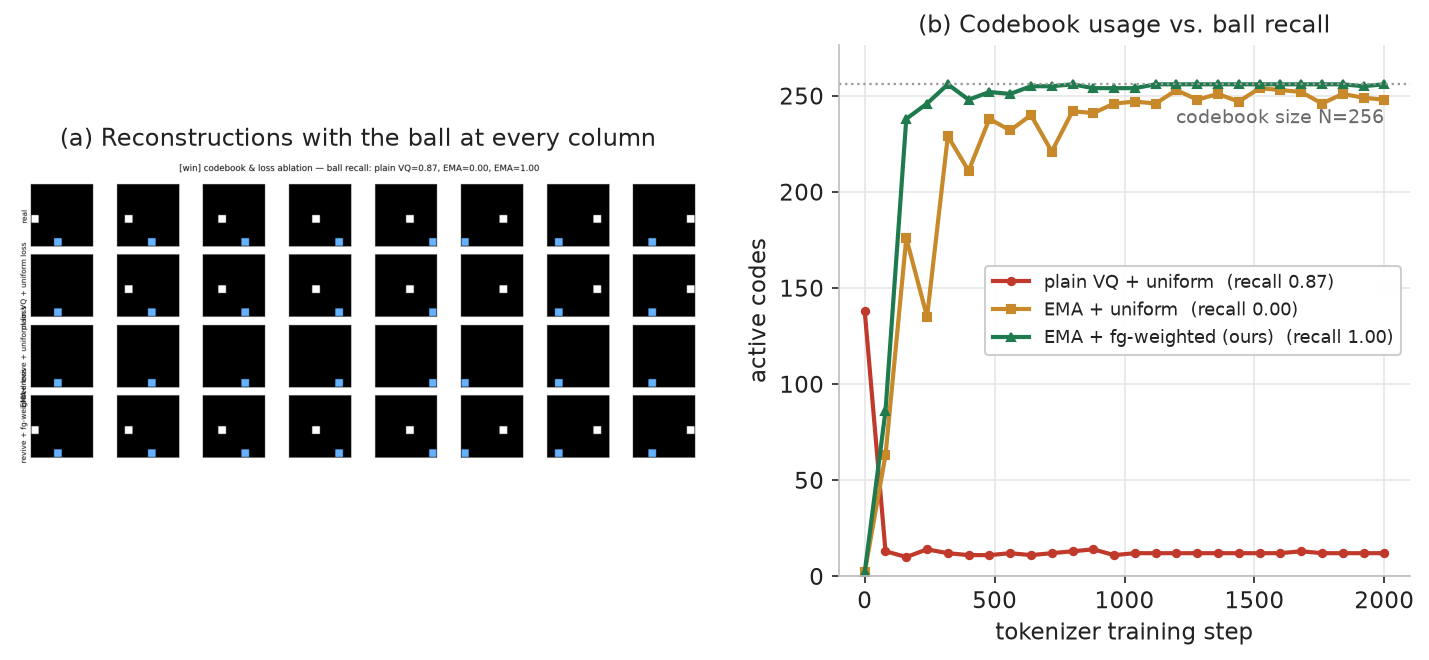
\includegraphics[width=\textwidth]{figures/fig_codebook_ablation.png}
\caption{(a) Reconstructions of frames with the ball at every column. Plain VQ and
EMA-with-uniform-loss both drop the white ball (keeping only the fixed blue
paddle); the foreground-weighted loss restores it. (b) Active codes over training:
EMA and EMA+fg keep the whole codebook alive, plain VQ collapses.}
\label{fig:ablation}
\end{figure}

\subsection{The world model: the easy part}
On the ball-preserving tokens the Transformer learns Catch's dynamics quickly:
\textbf{\wmTok\%} next-token accuracy, \textbf{\wmRew\%} reward accuracy, and
\textbf{\wmDone\%} done accuracy (Fig.~\ref{fig:wm}). Rolled forward under fixed
actions its dreams track the real environment closely
(Fig.~\ref{fig:wmreal})---and, unlike the base run, the dreamed frames now
\emph{contain the ball}, with a mean dream-vs-real MSE of \wmFidelity. Predicting a
discrete-token environment is what a Transformer is built for, and it shows.

\begin{figure}[H]\centering
\begin{minipage}{0.49\textwidth}\centering
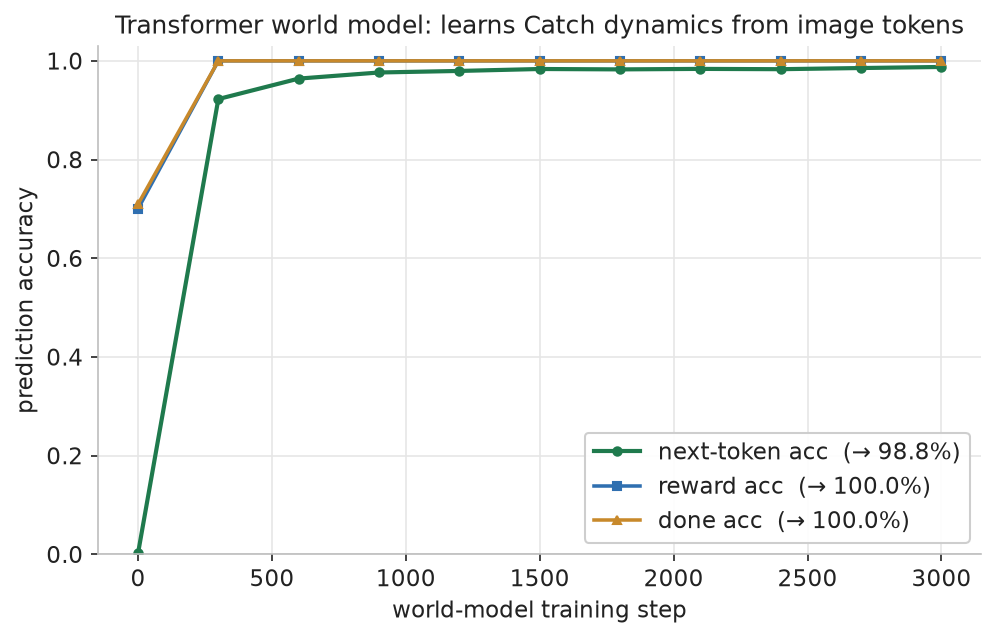
\includegraphics[width=\textwidth]{figures/fig_world_model.png}
\caption{World-model training: next-token, reward, and done accuracy all climb
rapidly.}\label{fig:wm}
\end{minipage}\hfill
\begin{minipage}{0.49\textwidth}\centering
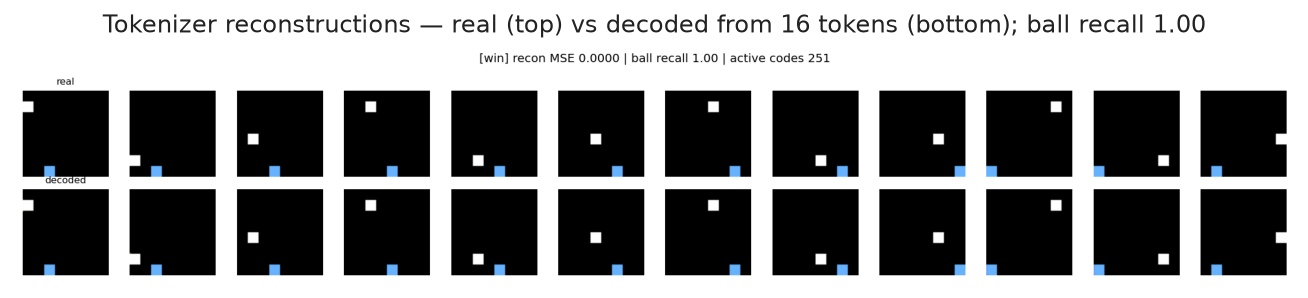
\includegraphics[width=\textwidth]{figures/fig_reconstruction_grid.png}
\caption{Tokenizer reconstructions with the fix: the ball is preserved at every
position (recall $\approx\!\ballFG$).}\label{fig:recon}
\end{minipage}
\end{figure}

\begin{figure}[H]\centering
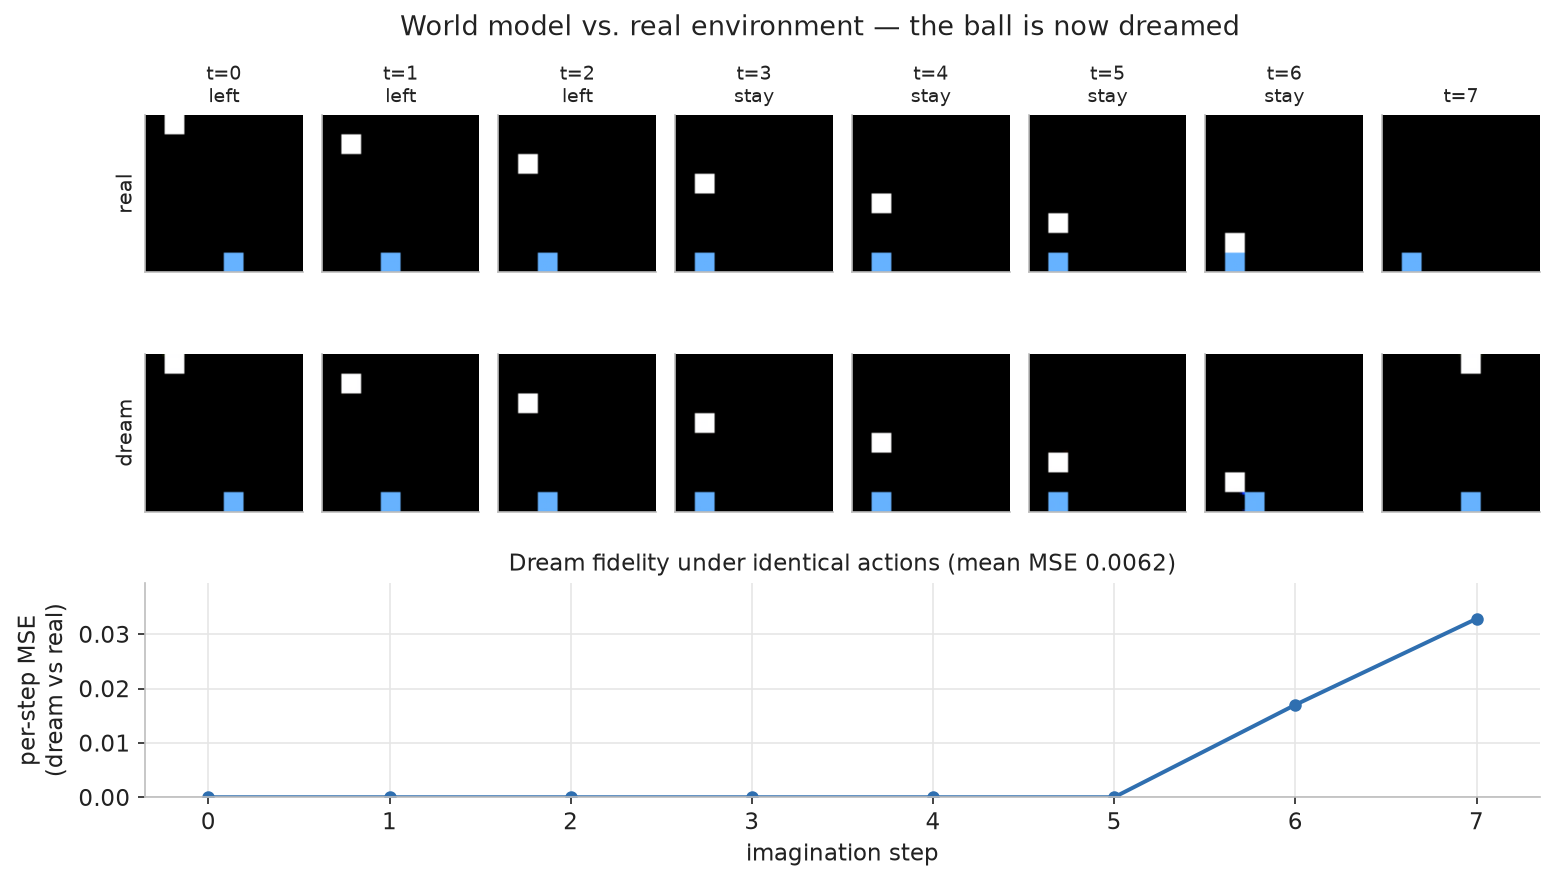
\includegraphics[width=0.95\textwidth]{figures/fig_wm_vs_real.png}
\caption{Real environment (top) vs.\ the world model's dream (bottom) under
identical actions, with per-step MSE. The dream now reproduces the falling ball
\emph{and} the moving paddle.}
\label{fig:wmreal}
\end{figure}

\subsection{The policy learns to catch}
\label{sec:policy-results}
With a dream that contains a ball, the actor-critic---trained \emph{only} on
world-model rollouts---learns to play. Its imagined return climbs out of negative
(random) territory into clearly positive values as the entropy bonus anneals and
the action distribution sharpens (Fig.~\ref{fig:policy}); the imagined return
plateaus below the real-environment optimum because it is measured under
stochastic sampling inside a slightly noisy dream, whereas evaluation uses the
greedy policy in the real environment. There, on $500$ fresh episodes, the policy
reaches a catch rate of \textbf{\catchRate} and mean return \catchReturn---%
\emph{matching the oracle} ($1.0$ / $+1.0$) and far above the random baseline
(\randCatch{} / \randReturn), Fig.~\ref{fig:baseline}. The dream filmstrips
(Fig.~\ref{fig:film}) show the learned paddle sliding under the ball and the
world model firing the terminal $+1$ reward---entirely in imagination.

\begin{figure}[H]\centering
\begin{minipage}{0.49\textwidth}\centering
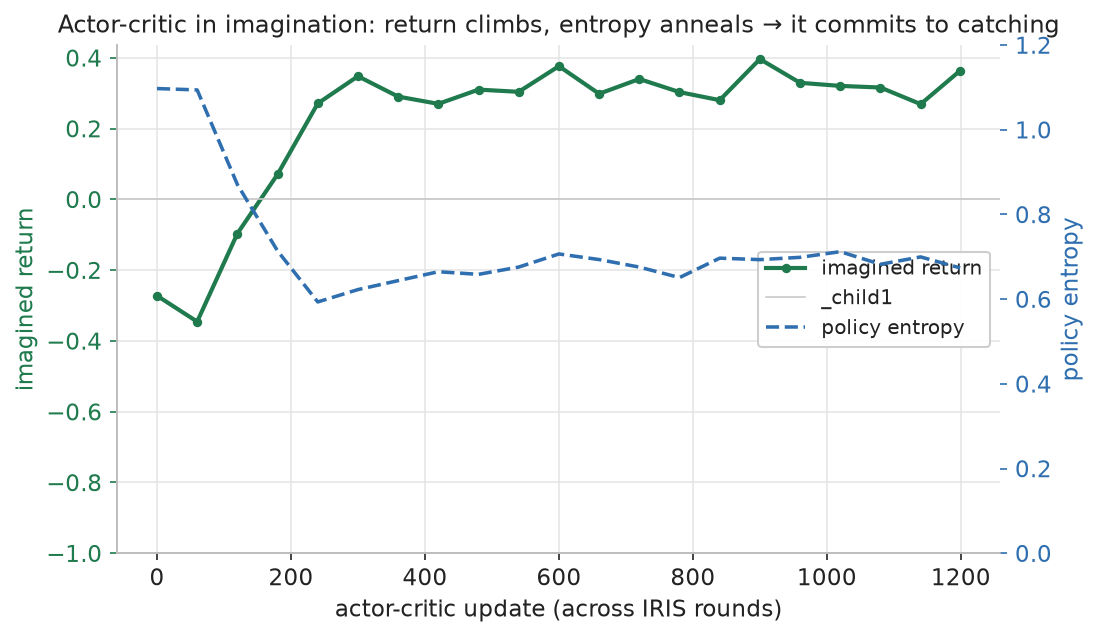
\includegraphics[width=\textwidth]{figures/fig_policy.png}
\caption{Actor-critic in imagination: imagined return climbs while entropy
anneals.}\label{fig:policy}
\end{minipage}\hfill
\begin{minipage}{0.49\textwidth}\centering
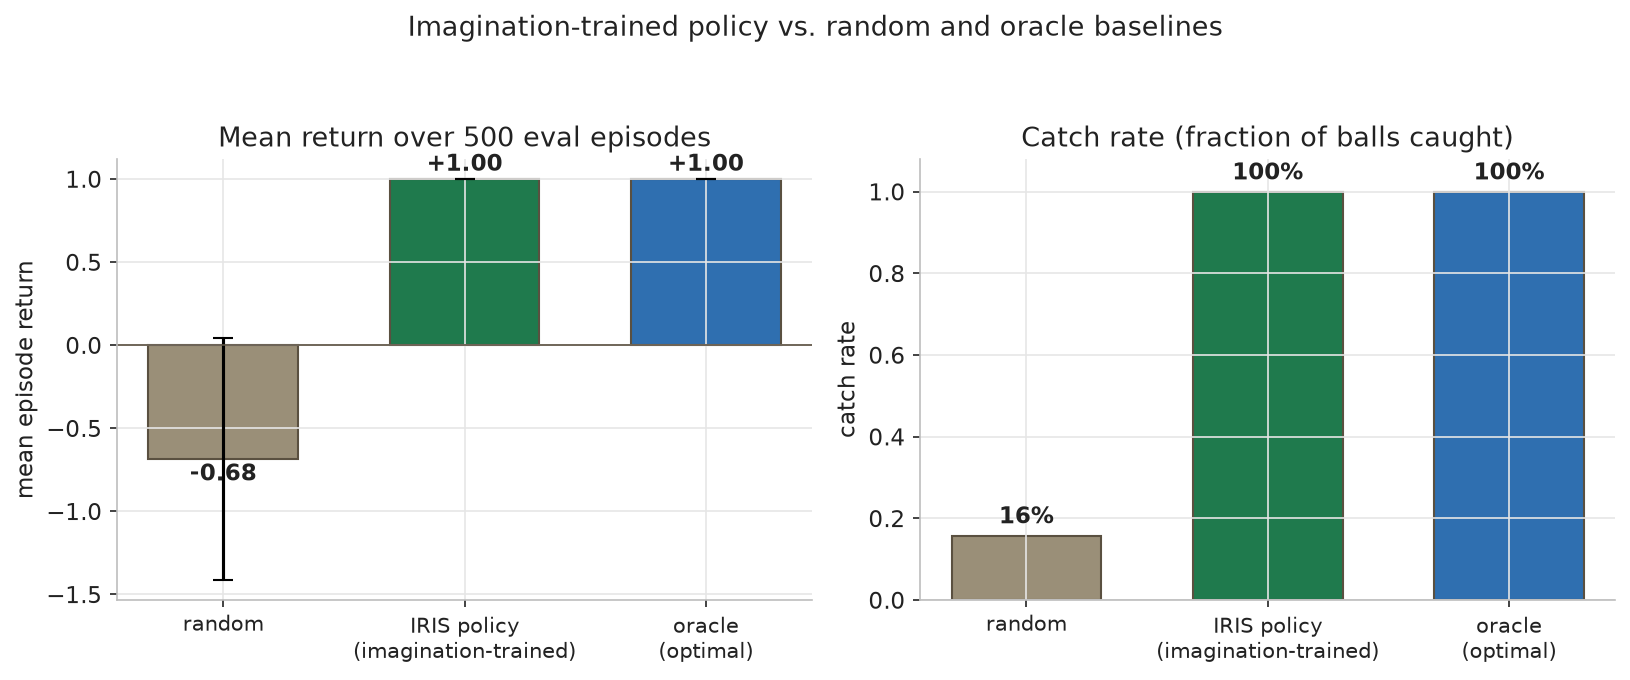
\includegraphics[width=\textwidth]{figures/fig_return_vs_baseline.png}
\caption{Evaluation over 500 real episodes: the imagination-trained policy vs.\
random and oracle.}\label{fig:baseline}
\end{minipage}
\end{figure}

\begin{figure}[H]\centering
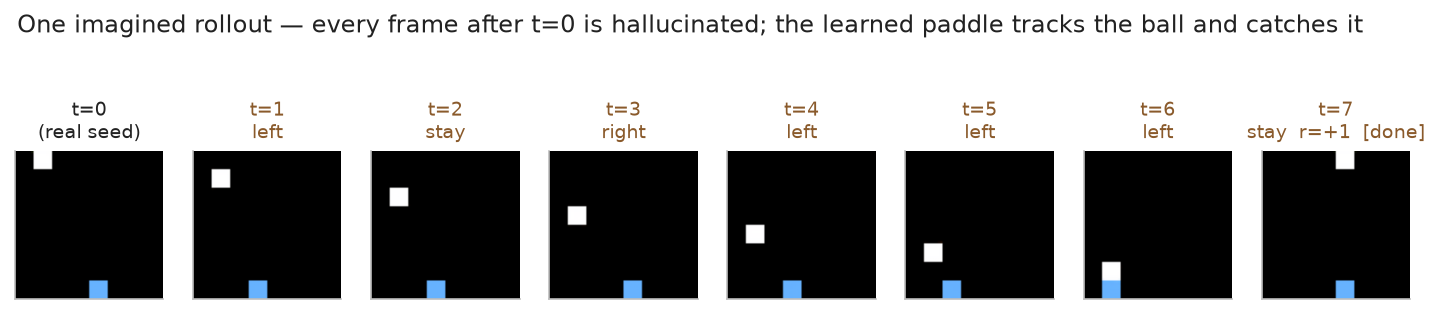
\includegraphics[width=0.95\textwidth]{figures/fig_dream_filmstrip.png}
\caption{One imagined rollout. Every frame after $t{=}0$ is hallucinated by the
world model; the learned paddle tracks the ball and the world model predicts the
terminal catch reward.}
\label{fig:film}
\end{figure}

\begin{table}[H]\centering
\caption{Scorecard after the fixes. Every number is from the real Modal run.}
\label{tab:scorecard}
\begin{tabular}{lrll}
\toprule
Component & Params & Headline metric & Verdict \\
\midrule
Tokenizer (VQ-VAE, ours) & \tokParams M & recon MSE $\reconFG$ / ball recall \ballFG & \textcolor{good}{\textbf{ball preserved}} \\
World model (Transformer) & \wmParams M & \wmTok\% next-token acc & \textcolor{good}{\textbf{works}} \\
Actor-critic (in dream) & \acParams M & catch rate \catchRate{} (random \randCatch) & \textcolor{good}{\textbf{learns to catch}} \\
\bottomrule
\end{tabular}
\end{table}

%============================================================================
\section{Discussion}
\label{sec:discussion}
%============================================================================
\paragraph{Codebook collapse is a red herring for the dropped ball.}
The most common explanation for a discrete autoencoder discarding content is
codebook collapse, and Table~\ref{tab:ablation} shows that collapse is indeed
real (plain VQ uses a small fraction of its codes). But the same table shows that
collapse does \emph{not} explain the missing ball: curing it with EMA and
dead-code revival restores a fully healthy \activeAfter-code codebook, yet the
ball is preserved in only \keptEMA{} of \nseeds{} seeds---no more reliably than
under the collapsed plain codebook. The decisive variable is the reconstruction
\emph{objective}. Holding the codebook mechanism fixed (EMA in both rows) and
changing only the loss---uniform vs.\ foreground-weighted---takes ball
preservation from \keptEMA/\nseeds{} to \keptFG/\nseeds{} seeds. A tokenizer
preserves what its loss rewards, and a uniform pixel loss barely rewards a ball
that is $0.5\%$ of the frame.

\paragraph{The coupling is the whole story.} These are not three independent
components that each happen to work or fail; they form a chain. Because the
tokenizer discarded the ball, the world model's dream contained nothing to catch;
because the dream had no ball, the reward head could not ground a catch/miss in
anything the agent \emph{sees}; because the reward was ungroundable, the policy
received no usable gradient and correctly settled at random. Fixing the tokenizer
is the first domino, and once it falls the rest follow with standard training.
This is why the naive agent looked like an RL failure when the real bug was three
stages upstream, in a reconstruction loss.

\paragraph{A cheap sanity check that would have caught it.} Before blaming the
policy, confirm that what the agent perceives is sufficient to predict the reward.
Our \textbf{ball-recall} probe---render frames with the object at known positions,
reconstruct, and measure whether it survives---is a two-minute, world-model-free
test that localizes the failure immediately. More generally: \emph{can a linear
probe on the tokens predict the reward?} If not, no amount of policy tuning will
help. This lesson transfers directly to Atari-scale MBRL, where the
task-critical objects (a bullet, a ball, a small enemy) are exactly the small,
fast, high-intensity structures a uniform reconstruction loss is happy to drop---
which is precisely why IRIS pairs its tokenizer with a perceptual loss.

\paragraph{Limitations.} Catch is deliberately minimal and deterministic; the
policy and world-model numbers are from a single run (the tokenizer ablation is
over $\nseeds$ seeds). The foreground-weighting trick exploits the fact that
salient objects here are bright; on natural images the perceptual loss it stands
in for is the more general instrument. Finally, the policy stage dominates
wall-clock, so the cheapest high-leverage intervention---as this paper
argues---is to get the representation right first, and only then spend compute on
the actor-critic.

%============================================================================
\section{Reproducibility}
\label{sec:reproduce}
%============================================================================
Every result is produced by a sequence of Modal (\url{https://modal.com})
entrypoints reading a
single YAML config (\texttt{configs/catch\_win.yaml}); the from-scratch model
code (\texttt{tokenizer.py}, \texttt{world\_model.py}, \texttt{actor\_critic.py},
\texttt{imagination.py}, \texttt{envs.py}) uses no external RL or \texttt{iris}
library.
\begin{verbatim}
modal run modal_apps/train.py::run_all  --cfg configs/catch_win.yaml --tag win
modal run modal_apps/evals.py::recon    --cfg configs/catch_win.yaml --tag win
modal run modal_apps/train.py::ablate   --cfg configs/catch_win.yaml --tag win
modal run modal_apps/evals.py::eval     --cfg configs/catch_win.yaml --tag win --n 500
modal run modal_apps/evals.py::dreams   --cfg configs/catch_win.yaml --tag win
modal run modal_apps/evals.py::sync
./.plotvenv/bin/python make_paper_figures.py
\end{verbatim}
The tokenizer fix is two config lines (\texttt{ema: true},
\texttt{fg\_weight: 25}); the ablation in \S\ref{sec:results} re-runs the
tokenizer with each turned off in turn, on the \emph{same} replay buffer, so the
before/after comparison is controlled.

%============================================================================
\section{Conclusion}
\label{sec:conclusion}
%============================================================================
Building all three IRIS components from scratch and running them on a real GPU
budget turns a model-based RL agent into something you can debug end-to-end. The
Transformer world model---the piece that sounds hardest---is the easy part: it
learns pixel-Catch to \wmTok\% token accuracy in under a minute of GPU time. The
genuinely hard part is upstream, in the discrete representation, and it hides a
trap that the usual ``codebook collapse'' diagnosis walks right past: a
background-dominated reconstruction loss silently discards small, fast,
task-critical objects, and a perfectly healthy codebook does nothing to stop it.
Naming that failure precisely---and fixing it with a one-line foreground-weighted
loss on top of standard EMA codebook updates---is what carries the agent from
random play (catch rate \randCatch) to a policy that learns entirely in
imagination (catch rate \catchRate, oracle $1.0$). \textbf{A world model can only
teach a policy what its tokenizer chooses to preserve.}

\begin{thebibliography}{10}
\bibitem{iris} V.~Micheli, E.~Alonso, and F.~Fleuret.
  Transformers are Sample-Efficient World Models.
  In \emph{ICLR}, 2023. arXiv:2209.00588.
\bibitem{worldmodels} D.~Ha and J.~Schmidhuber.
  World Models. arXiv:1803.10122, 2018. (NeurIPS 2018, ``Recurrent World Models
  Facilitate Policy Evolution.'')
\bibitem{dreamer} D.~Hafner, T.~Lillicrap, J.~Ba, and M.~Norouzi.
  Dream to Control: Learning Behaviors by Latent Imagination.
  In \emph{ICLR}, 2020. arXiv:1912.01603.
\bibitem{dreamerv2} D.~Hafner, T.~Lillicrap, M.~Norouzi, and J.~Ba.
  Mastering Atari with Discrete World Models.
  In \emph{ICLR}, 2021. arXiv:2010.02193.
\bibitem{dreamerv3} D.~Hafner, J.~Pasukonis, J.~Ba, and T.~Lillicrap.
  Mastering Diverse Domains through World Models. arXiv:2301.04104, 2023.
\bibitem{vqvae} A.~van den Oord, O.~Vinyals, and K.~Kavukcuoglu.
  Neural Discrete Representation Learning. In \emph{NeurIPS}, 2017.
  arXiv:1711.00937.
\bibitem{vqvae2} A.~Razavi, A.~van den Oord, and O.~Vinyals.
  Generating Diverse High-Fidelity Images with VQ-VAE-2.
  In \emph{NeurIPS}, 2019. arXiv:1906.00446.
\bibitem{jukebox} P.~Dhariwal, H.~Jun, C.~Payne, J.~W.~Kim, A.~Radford, and
  I.~Sutskever. Jukebox: A Generative Model for Music. arXiv:2005.00341, 2020.
\bibitem{simple} L.~Kaiser et al.
  Model-Based Reinforcement Learning for Atari. In \emph{ICLR}, 2020.
  arXiv:1903.00374.
\bibitem{bsuite} I.~Osband et al.
  Behaviour Suite for Reinforcement Learning. In \emph{ICLR}, 2020.
  arXiv:1908.03568.
\end{thebibliography}

\end{document}
